\subsection{Graphical User Interface}

\begin{figure}[h]
	\centering
	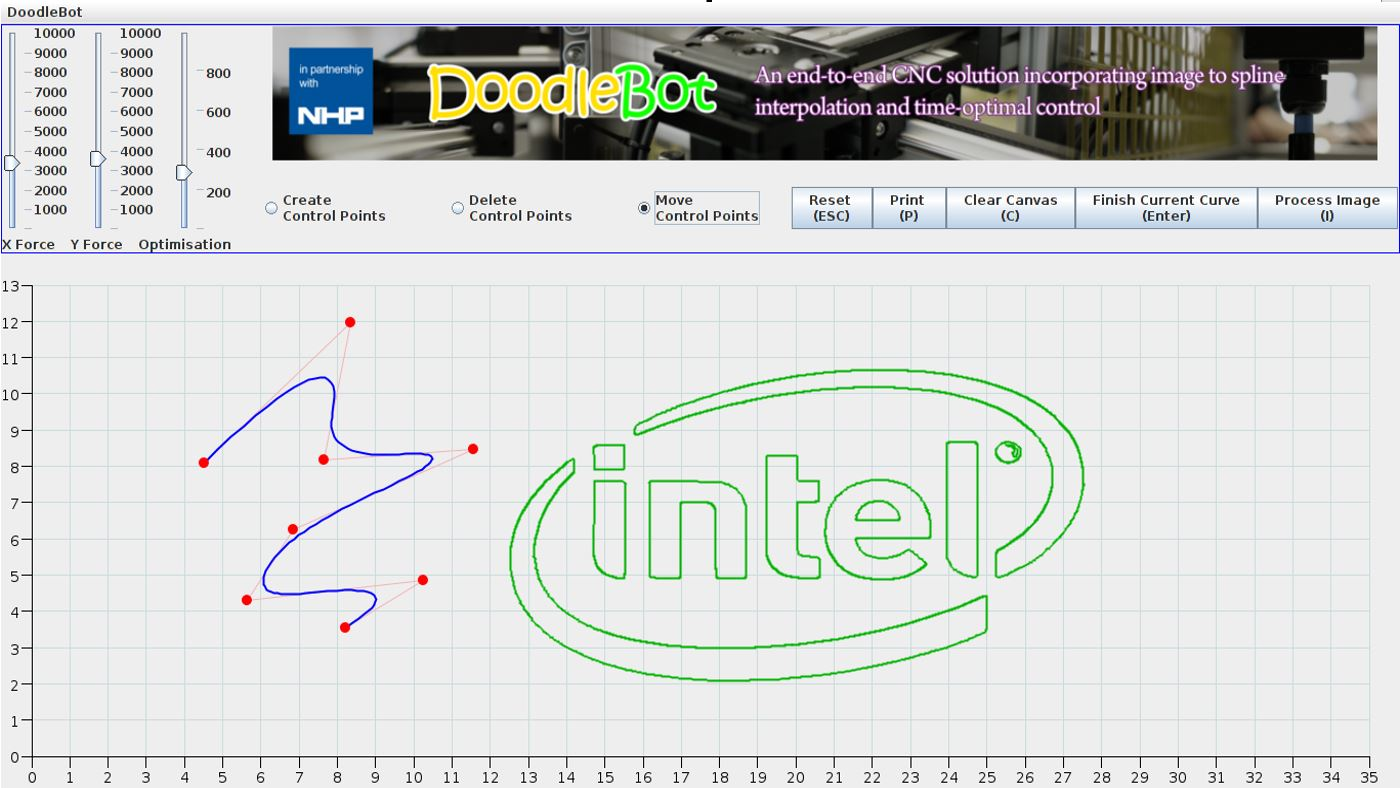
\includegraphics[width=\textwidth]{figures/implementation/interface.jpg}
	\caption[The DoodleBot GUI]{The DoodleBot GUI with both manually drawn URBS and an interpolated image file}
	\label{fig:guiscreen}
\end{figure}

The Graphical User Interface (GUI), shown in Figure ~\ref{fig:guiscreen}, is the input mechanism for the user. The GUI renders and displays a buffered collection of URBS curves and allows the user to add to this input buffer. When the user desires to print the buffered curves, the GUI hands the input buffer over to the MATLAB\textsuperscript{\textregistered} optimisation algorithm and adds the printed curves to a separate 'printed' buffer, which displays the processed curves in a different colour. The user can then continue to add curves to the input buffer and repeat the input process.

Addition to the input buffer occurs in two ways. Firstly, the user can select an image to render into splines. This opens a file selection dialogue, which will run the MATLAB\textsuperscript{\textregistered} image processing script upon the selection of an appropriate image. The script returns a set of URBS curves, which are added to the input buffer and displayed to the user as if they had entered the curves themselves.

The other input mechanism is manual spline creation, where the user can input the control points of a URBS curve themselves. The user can manipulate the positions of existing control points, add more control points or delete control points- with the rendering of the URBS curve updating in real time. After the user is satisfied with their curve, they can place it into the input buffer and continue to manipulate further curves.

When the user is satisfied with a scene, they can order the GUI to print the URBS input buffer. This places the generated URBS curves into the printing pipeline, which results in the curves getting printed by the DoodleBot.

There are several control functions for the clearing of buffers and resetting of the server queue available for the user. This enables the user to cancel operations that are in progress, or clear the currently displayed buffer to start the input process over again.